%-*-coding: utf-8-*-

\FloatBarrier
\chapter{Примеры полученных решений} \label{AppendixA}

\begin{figure}[h!]
  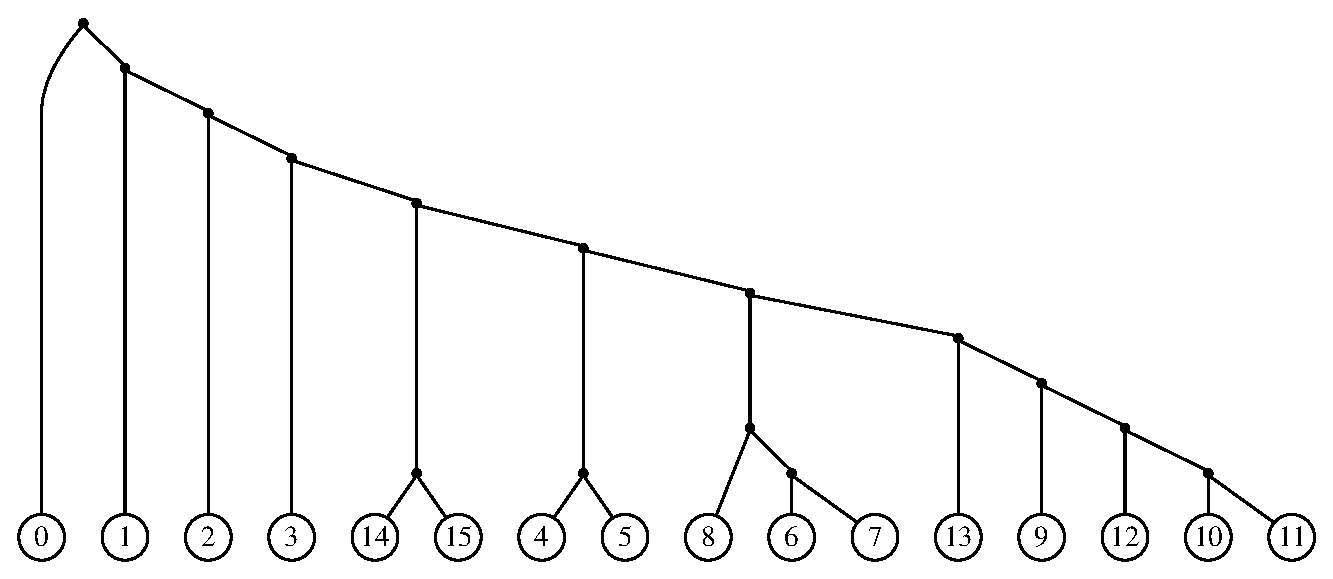
\includegraphics[width=\linewidth]{img/Grass2WaxyIts_tree0}
  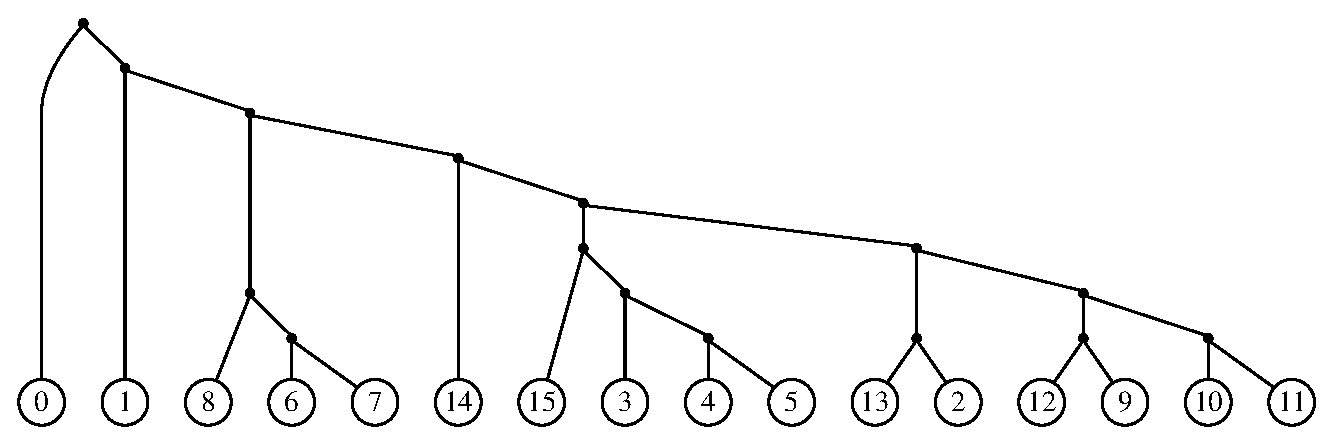
\includegraphics[width=\linewidth]{img/Grass2WaxyIts_tree1}
  \\\\\\
  \centering
  Рис. 1.1: Входные деревья для теста WaxyIts.
\end{figure}

\begin{figure}[h]
  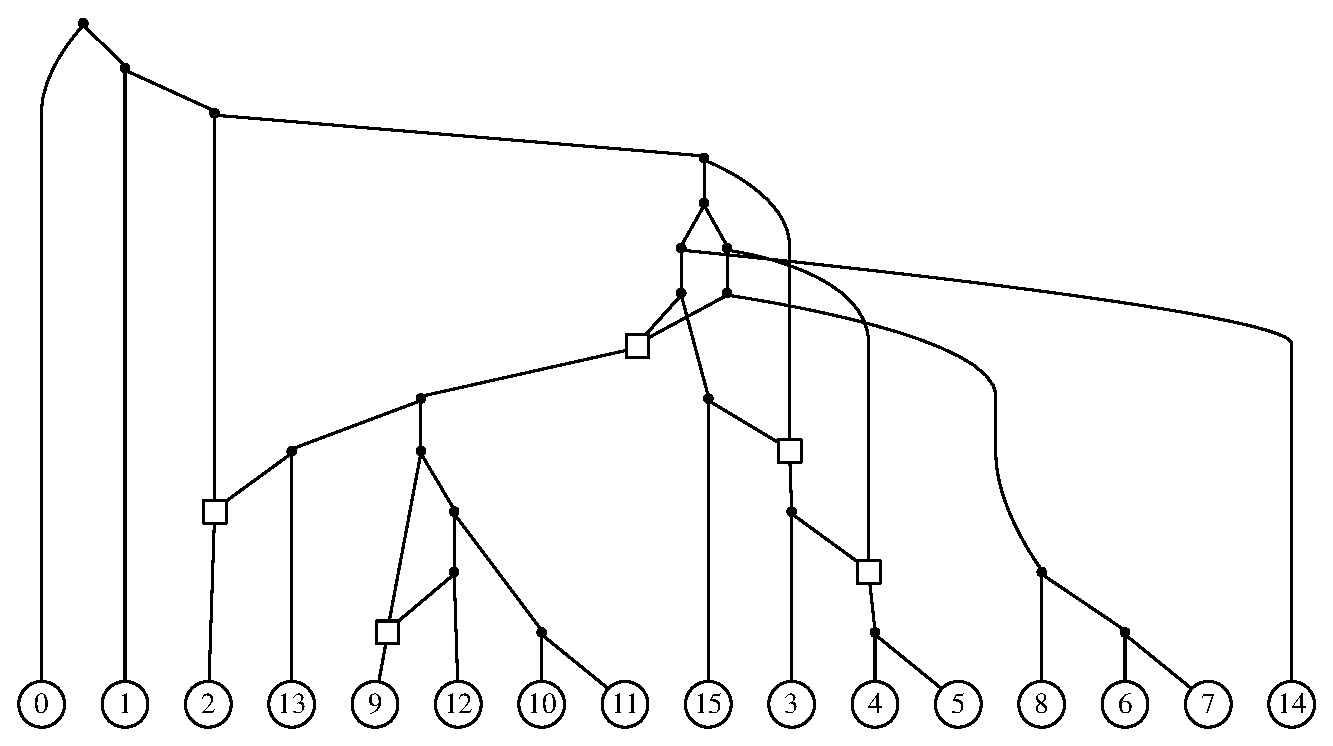
\includegraphics[width=\linewidth]{img/Grass2WaxyIts}
  \\\\\\
  \centering
  Рис. 1.2: Минимальная гибридизационная сеть для теста WaxyIts.
\end{figure}

\begin{figure}[h]
  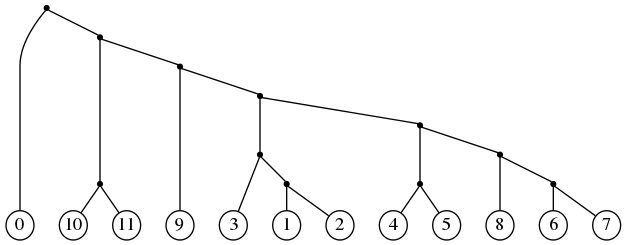
\includegraphics[width=\linewidth]{img/Grass3RbclWaxyIts_tree0}
  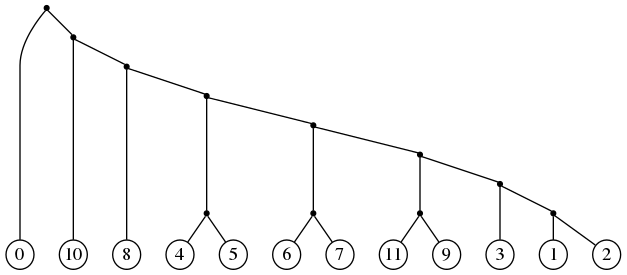
\includegraphics[width=\linewidth]{img/Grass3RbclWaxyIts_tree1}
  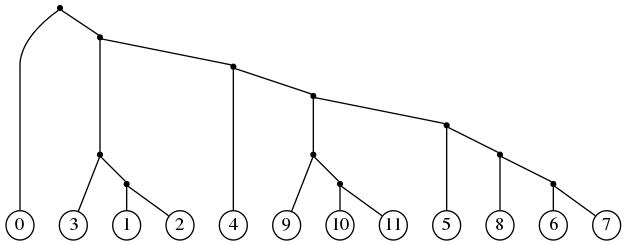
\includegraphics[width=\linewidth]{img/Grass3RbclWaxyIts_tree2}
  \\\\\\
  \centering
  Рис. 1.3: Входные деревья для теста RbclWaxyIts.
\end{figure}

\begin{figure}[h]
  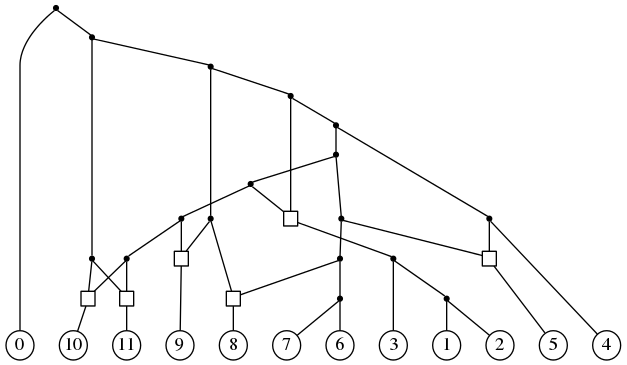
\includegraphics[width=\linewidth]{img/Grass3RbclWaxyIts}
  \\\\\\
  \centering
  Рис. 1.4: Минимальная гибридизационная сеть для теста RbclWaxyIts.
\end{figure}

\chapter{Подробные результаты тестирования} \label{AppendixB}

\begin{table}[h!]
Таблица 2.1: Подробные результаты тестирования PhyloSAT и PIRN$\mathrm{_{CH}}$. Приведены гибридизационные числа итоговых сетей. -1 означает, что не было получено никакой сети.
\\\\\\
\centering
\resizebox{0.55\textwidth}{!}{  
\begin{tabular}{l|c|c|c|c}
& PhyloSat & Время (сек) & PIRN$\mathrm{_{CH}}$ & Время (сек) \\
\hline
NdhfIts             & -1       & 1000  & -1   & 1000  \\
NdhfPhyt            & 8        & 11    & -1   & 1000  \\
NdhfRbcl            & 8        & 1     & 8    & 856   \\
NdhfRpoc            & 9        & 953   & 9    & 485   \\
NdhfWaxy            & 6        & 9     & 6    & 6     \\
PhytIts             & 8        & 45    & 8    & 373   \\
PhytRbcl            & 4        & 0     & 4    & 3     \\
PhytRpoc            & 4        & 0     & 4    & 1     \\
PhytWaxy            & 3        & 0     & 3    & 0     \\
RbclIts             & -1       & 1000  & -1   & 1000  \\
RbclRpoc            & 7        & 1000  & 7    & 43    \\
RbclWaxy            & 4        & 4     & 4    & 0     \\
RpocIts             & -1       & 1000  & -1   & 1000  \\
RpocWaxy            & 2        & 0     & 2    & 0     \\
WaxyIts             & 5        & 8     & 5    & 2     \\
NdhfPhytIts         & 13       & 1000  & -1   & 1000  \\
NdhfPhytRbcl        & 9        & 100   & -1   & 1000  \\
NdhfPhytRpoc        & 8        & 1000  & 8    & 28    \\
NdhfPhytWaxy        & 4        & 0     & 4    & 1     \\
NdhfRbclIts         & -1       & 1000  & -1   & 1000  \\
NdhfRbclRpoc        & 12       & 1000  & -1   & 1000  \\
NdhfRbclWaxy        & 5        & 67    & 5    & 0     \\
NdhfRpocIts         & -1       & 1000  & -1   & 1000  \\
NdhfRpocWaxy        & 3        & 0     & 3    & 0     \\
NdhfWaxyIts         & 8        & 1000  & 8    & 89    \\
PhytRbclIts         & 9        & 1000  & 8    & 116   \\
PhytRbclRpoc        & 6        & 12    & 6    & 3     \\
PhytRbclWaxy        & 2        & 0     & 2    & 0     \\
PhytRpocIts         & 7        & 1000  & 7    & 58    \\
PhytWaxyIts         & 4        & 0     & 4    & 0     \\
RbclRpocIts         & -1       & 1000  & -1   & 1000  \\
RbclRpocWaxy        & 3        & 0     & 3    & 0     \\
RbclWaxyIts         & 6        & 1000  & 7    & 3     \\
RpocWaxyIts         & 4        & 2     & 4    & 0     \\
NdhfPhytRbclIts     & -1       & 1000  & -1   & 1000  \\
NdhfPhytRbclRpoc    & 9        & 1000  & 10   & 279   \\
NdhfPhytRbclWaxy    & 2        & 0     & 2    & 0     \\
NdhfPhytRpocIts     & 10       & 1000  & -1   & 1000  \\
NdhfPhytWaxyIts     & 5        & 0     & 5    & 15    \\
NdhfRbclRpocIts     & -1       & 1000  & -1   & 1000  \\
NdhfRbclRpocWaxy    & 4        & 1     & 4    & 0     \\
NdhfRbclWaxyIts     & 6        & 1000  & 7    & 35    \\
NdhfRpocWaxyIts     & 5        & 42    & 5    & 2     \\
PhytRbclRpocIts     & 9        & 1000  & 8    & 364   \\
PhytRbclWaxyIts     & 2        & 0     & 2    & 0     \\
RbclRpocWaxyIts     & 5        & 34    & 5    & 2     \\
NdhfPhytRbclRpocIts & -1       & 1000  & -1   & 1000  \\
NdhfPhytRbclWaxyIts & 3        & 0     & 3    & 0     \\
NdhfRbclRpocWaxyIts & 5        & 34    & 5    & 13    \\
\end{tabular}
}
\end{table}
